\section{1174002 - Habib Abdul Rasyid}

\subsection{Teori}
\subsubsection{Definisi Kecerdasan Buatan}
\hfill\break
Kecerdasan buatan atau artificial intelligence (AI) menurut beberapa pakar adalah sebagai berikut:
\begin{enumerate}

\item Definisi Sejarah Kecerdasan Buatan

Kecerdasan buatan atau yang dikenal dengan Artificial Intelligence (AI) adalah suatu perkembangan teknologi yang muncul untuk membentuk suatu mesin teknologi yang lebih pintar yang mana agar lebih memudahkan setiap pekerjaan manusia. Selain itu AI ini juga untuk memahami kecerdasan dalam artian membuat sebuah mesin yang dapat membantu memahami kecerdasan contohnya dapat memcahkan sebuah masalah dengan lebih cepat.

\item Definisi Kecerdasan Buatan

Kecerdasan buatan atau yang disebut dengan Artificial Intelligence mulai muncul sekitar tahun 1940 dan 1950 sejak adanya komputer. Munculnya AI ini memberikan banyak keuntungan seperti AI ini berisfat permanen, artinya bisa digunakan secara berulang-ulang dimana saja dan kapan saja. Selain itu menawarkan kemudahan dalam artian data yang telah disimpan sebelumnya akan mudah untuk di akses kembali. Kerja AI ini juga lebih cepat jika dibandingkan dengan kerja manusia


\item Definisi Perkembangan Kecerdasan Buatan
Tahun 1960 s/d 1970, mulailah berbagai diskusi tentang bagaimana komputer dapat menirukan dengan sedetail mungkin kemampuan otak manusia, saat itu dikategorikan dengan "classical AI". Kemudian pada tahun 1980, saat itu komputer sudah mudah didapatkan dengan harga yang terjangkau yang memudahkan berbagai riset dibidang kecerdasan buatan berkembangan dengan pesat diu berbagai universitas dunia.\\

John McCarthy dari Massacuhetts Institute of Technology atau yang dikenal sebagai Bapak AI, pada tahun 1956 McCarthy mengadakan konferensi Dartmouth Workshop yang melahirkan suatu bidang baru dengan nama “Artificial Intelligence". Pada konferensi Dartmouth itu mempertemukan semua para pendiri AI, dimana John McCarthy yang mengusulkan defisi dari AI itu. AI adalah cabang dari ilmu komputer yang berfikus pada pengembangan komputer yang dapat memiliki kemampuan layakntya manusia.

\item Definisi supervised learning 
Supervised learning mempunyai input dan output yang bisa dibuat menjadi model hubungan matematis, dan juga sebuah pendekatan dimana sudah terdapat data yang dilatih selain itu juga ada sebuah variable yang sudah ditargetkan sebagai tujuan dari pendekatan ini yaitu pengelompokan data ke data yang sudah ada sebelumnya.\\
Pengertian dalam konteks AI, supervised learning adalah sistem dimana sebuah input dan output data yang kita inginkan sudah tersedia. Input dan output data ini diberi label untuk klasifikasi dasar pembelajaran untuk pemrosesan data yang akan datang. Supervised learing ini menyediakan algoritma untuk pembelajaran dengan jumlah diketahui untuk mendukung sebuah penilaian yang akan datang seperti: Regrasi Linear Berganda, Analisis Deret Waktu, Decision tree dan Random Forest, Artificial Neural Network, dan lain sebagainya.

\item Definisi Klasifikasi
Klasifikasi merupakan sebuah proses pengelompokan benda berdasarkan ciri-ciri persamaan dan perbedaan. Artinya kita memberitahu mesin tersebut bagaimana cara pengerjaannya berdasarkan kelompok.

\item Definisi Regrasi
Regrasi adalah bagian dari problem Supervised Learning, regrasi ini menggunakan metode statistika.

\item Definisi Unsupervised Learning
Unsupervised Learning berbeda dengan suprevised learning. Unsupervised Learning tidak memiliki data latih, sehingga dari data yang telah ada kita kelompokkan menjadi dua atau tigas bagian begitupun seterusnya. Unsupervised Learning ini merupakan pelatihan algoritma kecerdasan buatan emnggunakan informasi yang tidak diklasifikasikan atau diberi label dan memungkinkan algoritma untuk bertindak atas informasi tersebut tanpa panduan. \\
Tujuan dari algoritma tersebut adalah untuk mengelompokkan sebuah objek yang hampir mirip atau sama ke dalam area tertentu

\item Definisi Data Set
Dataset merupaskan objek yang merepresentasikan sebuah data dan relasi yang ada di memory. Struktur data set mirip dengan data yang ada didalam sebuah database.Namun, didalam dataset berisi sebuash koleksi dari data tabel dan data relation.
\item Definisi Training Set
Traning set merupakan set yang digunakan oleh algoritma klassifikasi. Contohnya adalah decision tree, bayesian, neural network, dan lain sebagainya.

\item Testing Set
Testing set merupakan sebuah set yang digunakan untuk mengukur sejauh mana sebuah classfier berhasil melakukan klasifikasi dengan benar. Testing set berfungsi sebagai materai persetujuan, tapi tidak dapat kita gunakan sampai akhir. Setelah data di optimalkan, kita dapat melakukan pengujian jaringan saraf terhadapt pengambilan sampel acak. Kemudian hasil yang diperolah harus valid bahwa jaringan kita akurat dalam menegnali gambar.\\

\end{enumerate}
\subsection{Praktek}
\begin{enumerate}
	\item Instalasi  library  scikit  dari  anaconda,  mencoba  kompilasi  dan  uji  coba  ambil contoh kode dan lihat variabel explorer.
	
	\textbf{Instalasi Library Scikit-Learn dengan Anaconda}
	\begin{enumerate}
		\item Pertama pastikan anda telah menginstall Anaconda. Jika sudah menginstall Anaconda, jalankan Anaconda Navigator.
		\begin{figure}[H]
			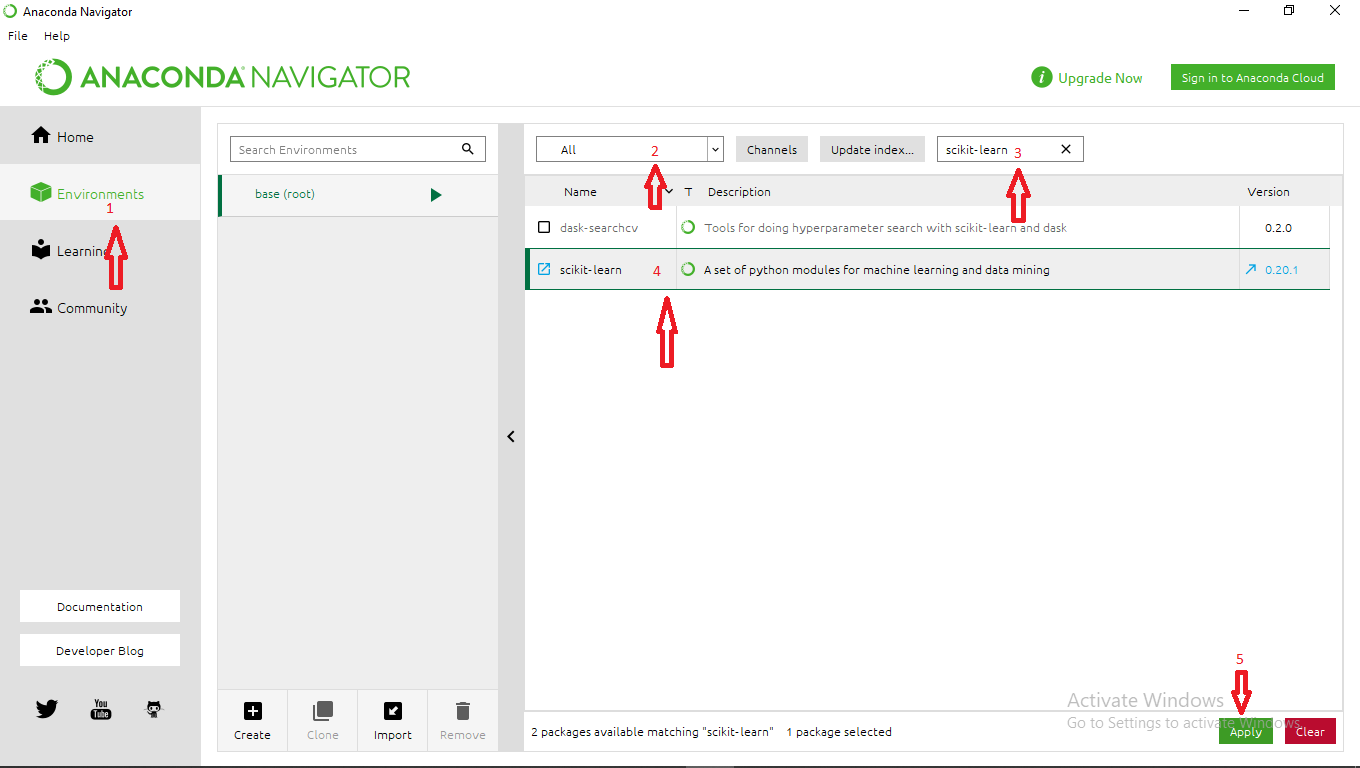
\includegraphics[width=1\textwidth]{figures/1174002/chapter1/praktek/ins.png}
			\centering
			\caption{Instalasi Library Scikit-Learn.}
		\end{figure}
		\item Pilih menu Environment.
		\item Kemudian pada filter pilih menu semua atau all.
		\item Setelah itu cari scikit-learn di kolom pencarian.
		\item Selanjutnya centang library scikit-learn, lalu klik tombol Apply.
	\end{enumerate}

	\textbf{Mencoba Menggunakan Library scikit-Learn}
	\begin{enumerate}
		\item Pertama jalankan aplikasi Spyder.
		\item Kemudian buat file baru, lalu tambahkan kode berikut.
		\lstinputlisting[firstline=8, lastline=10]{src/1174002/chapter1/coba.py}
		\item Simpan dan jalankan.
		\item Hasil dari variabel explorernya sebagai berikut.
		\begin{figure}[H]
			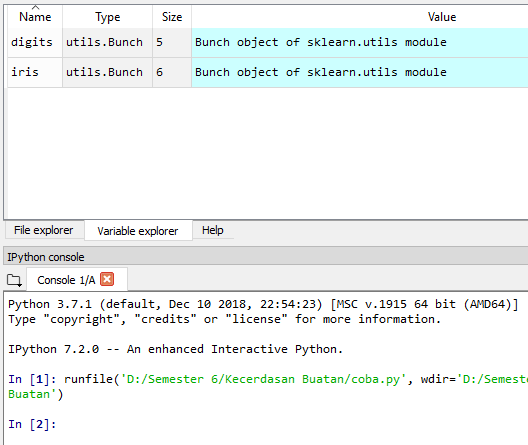
\includegraphics[width=1\textwidth]{figures/1174002/chapter1/praktek/hasil.png}
			\centering
			\caption{Variabel Explorer Library Scikit-Learn.}
		\end{figure}
	\end{enumerate}
	
	\item Mencoba Loading an example dataset, menjelaskan maksud dari tulisan terse-but dan mengartikan per baris.
	\lstinputlisting[firstline=12, lastline=16]{src/1174002/chapter1/coba.py}
	
	Hasilnya akan seperti ini.
	\begin{figure}[H]
		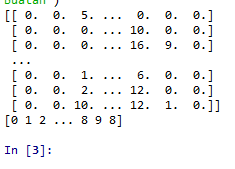
\includegraphics[width=5cm]{figures/1174002/chapter1/praktek/1.png}
		\centering
		\caption{Hasil Loading an Example Dataset.}
	\end{figure}

	\item Mencoba  Learning  and  predicting,  menjelaskan  maksud  dari  tulisan  tersebut dan mengartikan per baris.
	\lstinputlisting[firstline=17, lastline=22]{src/1174002/chapter1/coba.py}
	
	Hasilnya akan seperti ini.
	\begin{figure}[H]
		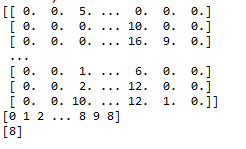
\includegraphics[width=1cm]{figures/1174002/chapter1/praktek/2.png}
		\centering
		\caption{Hasil Learning and Predicting.}
	\end{figure}

	\item Mencoba Model persistence, menjelaskan maksud dari tulisan tersebut dan mengartikan per baris.
	\lstinputlisting[firstline=23, lastline=39]{src/1174002/chapter1/coba.py}


	\item Mencoba Conventions, menjelaskan maksud dari tulisan tersebut dan mengartikan per baris.
	\lstinputlisting[firstline=41, lastline=87]{src/1174002/chapter1/coba.py}
	
	Hasilnya akan seperti ini.
	\begin{figure}[H]
		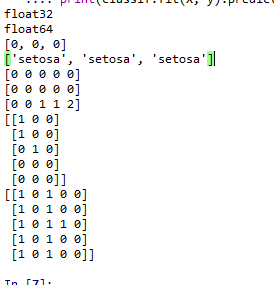
\includegraphics[width=5cm]{figures/1174002/chapter1/praktek/4.png}
		\centering
		\caption{Hasil Conventions.}
	\end{figure}

\end{enumerate}
\subsection{Penanganan Error}
\begin{enumerate}
	\item ScreenShoot Error
	\begin{figure}[H]
		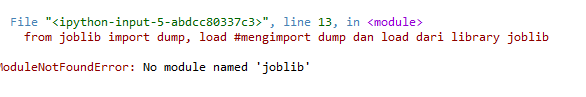
\includegraphics[width=4cm]{figures/1174002/chapter1/error/error.png}
		\centering
		\caption{Import Error}
	\end{figure}
	\item Tuliskan Kode Error dan Jenis Error
	\begin{itemize}
		\item Import Error
		\item Value Error
	\end{itemize}
	\item Cara Penangan Error
	\begin{itemize}
		\item Import Error
		\hfill\break
		Dengan Menginstall Library Yang Tidak Ditemukan
		\item Value Error
		\hfill\break
		Mengubah Bentuk Arraynya, Menjadi 1 Dimensi
	\end{itemize}
\end{enumerate}
\subsection{Bukti Tidak Plagiat}
\begin{figure}[H]
	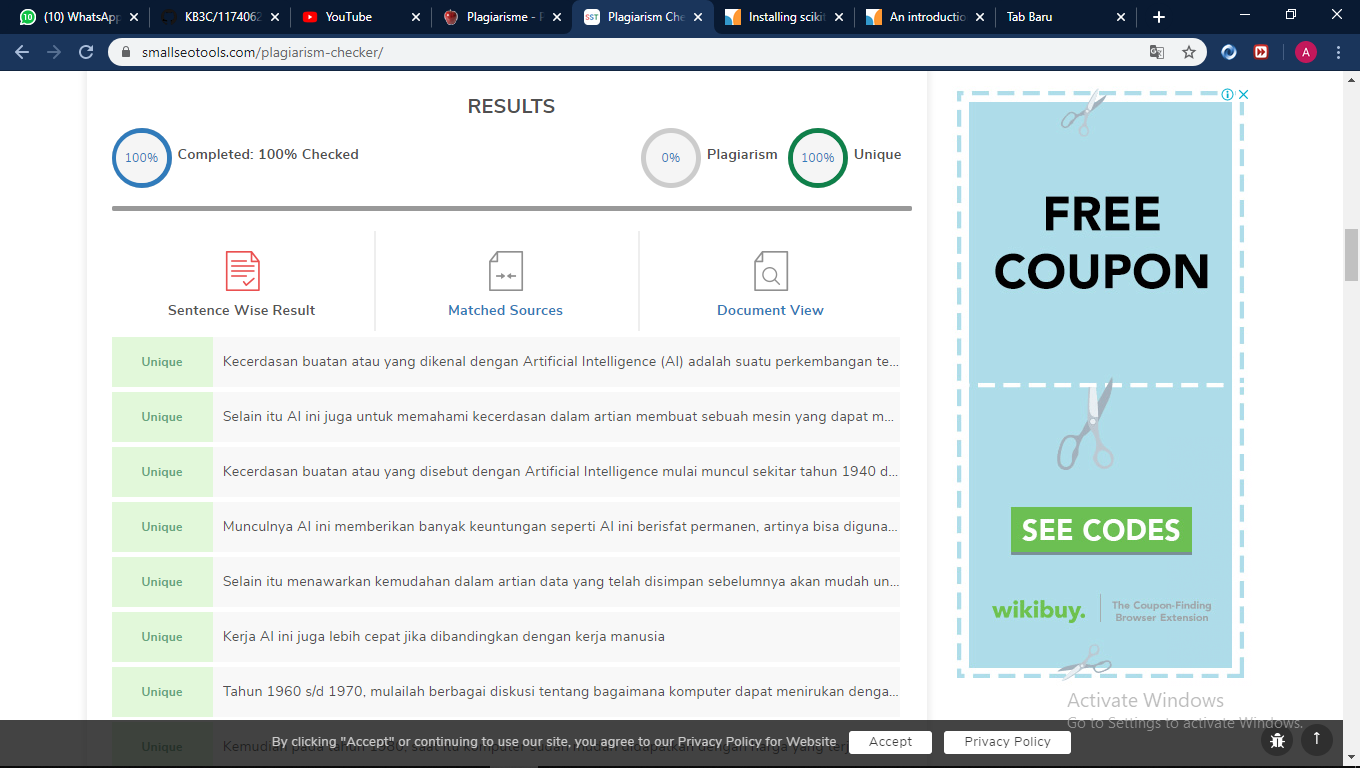
\includegraphics[width=4cm]{figures/1174002/chapter1/plagiat.PNG}
	\centering
	\caption{Bukti Tidak Melakukan Plagiat}
\end{figure}